\documentclass[11pt]{jreport}
\usepackage{wuse_thesis}
\usepackage{indentfirst}
\usepackage{url}	% \url{}コマンド用.URLを表示する際に便利
\usepackage{otf}
\usepackage{xcolor}
\usepackage[dvipdfmx]{graphicx}
\usepackage{enumitem}
%\usepackage{graphicx}  % ←graphicx.styを用いてEPSを取り込む場合有効にする
			% 他のパッケージ・スタイルを使う場合には適宜追加
            
\newcommand{\RQOne}{レビューコメントの中から修正要求を抽出することは可能か}
\newcommand{\RQTwo}{レビューコメントの中から修正確認を抽出することは可能か}
\newcommand{\RQThree}{コードレビュー票単位と修正要求単位に基づくタスクの完了状況評価結果は異なるか}

\newcommand{\todo}[1]{\colorbox{yellow}{{\bf TODO}:}{\color{red} {\textbf{[#1]}}}}
\newcommand{\change}[1]{\colorbox{green}{{\bf CHANGE}:}{\color{blue} {\textbf{[#1]}}}}
\newcommand{\new}[1]{\colorbox{cyan}{{\bf NEW}:}{\color{black} {\textbf{[#1]}}}}
%%%%%%%%%%%%%%%%%%%%%%%%%%%%%%%%%%%%%%%%%%%%%%%%%%%%%%%%%%%%%%%%%%%%%%%%

%%
%% 主に表紙を作成するための情報
%%

%%  タイトル(修論の場合は英語表記も指定)
\title{修正要求・確認コメントの自動抽出による\\
コードレビューのタスク完了状況追跡手法}
% \title{指導教員に才能を見出された俺、異世界でも無双する\\
% 〜魔王軍を討伐して最強パーティーを結成した件〜}
% \title{コードレビューって実際どうなってるの?\\
% 気になるよね?さあ!研究してみよう!\\
% 第1部! タスク管理ってだるい><\\
% 第2部! 俺ってもしかして最強?\\〜〜b4お前ら遅すぎてつまらん〜〜\\
% 第3部!  クリスマスイブに論文書く俺カッケー\\〜〜え?!裏切り者がいる!?〜〜\\
% 第4部! もう終わってるおれかっけー\\〜〜なんで君ら終わってないん?もう1ヶ月前やで??〜〜
% }

%%  著者名(修論の場合は英語表記も指定)
\author{川\UTF{FA11} 晴斗}
% \author{\todo{川\UTF{FA11} ラインハルト}}
%\eauthor{Akinori Ihara}

%% 卒業論文
\bachelar	% 卒業論文(4年生用)
% \master
%%  学科・クラスタ
\department{システム工}

%%  学生番号
\studentid{60266083}

%%  卒業年度
\gyear{2024}

%%  論文提出日
\date{2025年2月12日}
% \date{2027年2月12日}
%%%%%%%%%%%%%%%%%%%%%%%%%%%%%%%%%%%%%%%%%%%%%%%%%%%%%%%%%%%%%%%%%%%%%%%%

\begin{document}

\maketitle
% %-------------------
% \begin{center}
% \includegraphics[width=1.0\linewidth]{@BSthesis2024_Noguchi/Noguchi_fig/thank_irasutoya.pdf}
% \end{center}
% %-------------------
%%
%%  概要
%%

\begin{abstract}
本研究では,コードレビューにおけるレビューコメントがソフトウェアの開発プロセスに及ぼす影響を調査する.

ソフトウェア開発において,検証者は実装者が提出したソースコードに対して,可読性や欠陥の有無の確認を行い,次回のリリースへの導入の可否を決定する.大規模プロジェクトでは実装者から提出されるソースコードが膨大であるため,従来研究ではソースコードが提出された際にコードレビューの優先順位や工数の見積もりを行う手法を提案している.しかし,コードレビューにおいて,検証者と実装者の間でソースコードの修正に関する意見が対立し,予定時間を超過することも多い.

本研究では,レビューコメントの内容を詳細に分析し,個々のコードレビューのタスクの完了状況を追跡する手法を提案する.具体的には,ソースコードの修正を要求するコメント(修正要求コメント)と修正完了を確認するコメント(修正確認コメント)を自動で抽出し,これらを対応づけることで,各修正要求の対応状況を追跡する.

提案手法の有効性を検証するため,まず自然言語処理モデルのBERTとパターンマッチを用いて修正要求と修正確認の自動抽出を試みた.その結果,修正要求についてはF1値0.81,修正確認についてはF1値0.96という高精度での抽出が可能であることを確認した.次に,時系列に基づいて修正要求と修正確認の紐付けを行った結果,修正要求の86.6\%について対応する修正確認との紐付けに成功した.

本手法により,従来は困難であった個々のコードレビューのタスクの完了状況を詳細に追跡することが可能となり,ソフトウェアの開発プロセスの効率化に寄与することが期待される.

% \todo{SIGSEコピペ(OSSについて詳しくない人でもわかりやすく書く)}
% コードレビュー対象のソースコードが改善を要する場合,検証者は実装者に修正を要求する.ソフトウェア開発においてプロジェクト管理者は,コードレビューの進捗を確認しながら次のリリースに導入可能なソースコードを決定する.しかし大規模なプロジェクトでは,膨大なコードレビューが並行で進められ,個々の進捗を確認することは容易ではない.本研究では,レビューコメントから修正要求コメント,および修正要求が解決されたことを示す修正確認コメントをそれぞれ自動抽出し,コードレビューの進捗状況を追跡する手法を提案する.
\end{abstract}

%%  目次
\tableofcontents

%%  図目次 (図目次をいれたければ以下のコメントをはずす)
%\listoffigures

%%  表目次 (表目次をいれたければ以下のコメントをはずす)
%\listoftables

\newpage
\pagenumbering{arabic}	% 以降のページ番号を算用数字に

%%%%%%%%%%%%%%%%%%%%%%%%%%%%%%%%%%%%%%%%%%%%%%%%%%%%%%%%%%%%%%%%%%%%%%%%

%%
%%  本文はここから
%%

%%%%%%%%%%%%%%%%%%%%%%%%%%%%%%%%%%%%%%%%%%
%1章 はじめに
\chapter{はじめに}\label{chap:intro}
%%%%%%%%%%%%%%%%%%%%%%%%%%%%%%%%%%%%%%%%%%

\change{文同士の繋がりと接続詞を修正}

オープンソースソフトウェア(OSS: Open Source Software)は,著作権者が定めたライセンスによってソフトウェアの変更・配布の権利が規定され,ソースコードが公開されているソフトウェアである.OSSのソースコードは,そのライセンスの条件下で,誰でも自由に利用,修正,機能の拡張,再配布を行うことが可能である\cite{oss}.

不特定多数の実装者が参加するOSS開発では複数の開発者(実装者)がソフトウェアの機能の追加や不具合修正のために,変更したソースコードをプロジェクトに提出する.変更したソースコードは別の開発者(検証者)によってコードレビューが実施される.コードレビューは変更したソースコードに欠陥の有無やコードの可読性を損失する箇所が存在しないかを確認する重要な工程である\cite{quality1}\cite{quality2}.コードレビューによってソースコードの改善を要する箇所が発見されれば,検証者は実装者に改善を要求する. 

さらに,コードレビューはプロジェクトのリリースに直接影響を与える重要な要素の一つである.コードレビューの議論を通じて,変更されたソースコードがプロジェクトへの導入に適した水準を満たしていると判断された場合,次回のリリースへの導入が決定される.ソフトウェア開発プロジェクトでは,リリースまでのマイルストーンを計画するために,コードレビューを含めた各タスクの進捗を計画し,完了状況を追跡する必要がある\cite{review_time}.この進捗確認のため,ソースコードの共有や管理を行うサービスであるGitHub\footnote{GitHub: \url{https://github.co.jp/}}はMilestone機能を提供している.この機能により,特定の期限までに完了すべきコードレビュー(Pull Request)票の件数を把握することが可能となり,多くの組織がリリースまでのマイルストーン管理に活用している.ただし,コードレビューの過程では,実装者と検証者の間でソースコードの修正の必要性について対立することが多い\cite{review_time1}\cite{review_time2}.そのため,緻密なマイルストーンを計画するためには,個々のコードレビュー票に含まれるレビューの進捗状況を正確に追跡する必要がある.しかしながら,OSS開発では提出されるコードレビュー票が膨大であるため,個々のコードレビュータスクの完了状況を追跡することは困難である.

本研究では,コードレビューにおけるタスクの完了状況の把握に向けて,実装者と検証者の議論の中から,検証者がコードレビューによって更なる修正を依頼するコメント(修正要求コメント),及びソースコードが修正されたことを検証者が確認したことを伝えるコメント(確認コメント)を自動抽出する手法を提案する.また,GitHubのMilestoneのようにコードレビュー票単位でのタスクの完了状況追跡手法と,本研究で開発する修正要求単位でのタスクの完了状況追跡手法の違いを示す.

\noindent\textbf{RQ1: \RQOne (\ref{chap:RQ1}章)}\\
RQ1では,検証者が記録するコードレビュー票に残したコメントを修正要求に分類できるか否かを調査する.具体的には,OSS開発で公開されているコードレビュー票を無作為に抽出し,各コードレビュー票に記録されたレビューコメントを目視,及び機械的に分類を行う.

\noindent\textbf{RQ2: \RQTwo (\ref{chap:RQ2}章)}\\
RQ2では,検証者が記録するコードレビュー票に残したコメントを修正確認に分類できるか否かを調査する.具体的には,RQ1で無作為に抽出したコードレビュー票において,各コードレビュー票に記録されたレビューコメントを目視,及び機械的に分類を行う.

\noindent\textbf{RQ3: \RQThree (\ref{chap:RQ3}章)}\\
RQ3では,修正要求コメントとその要求が解決されたことを確認する修正確認コメントの紐付けを試みる.また,本研究で開発した修正要求コメント,及び修正確認コメントの抽出によってコードレビューのタスクの完了状況の追跡結果の違いを示す.

以降,本論文では,\ref{chap:review_process}章でOSS開発におけるコードレビューと従来研究について述べる.その後,\ref{chap:case_study}章で本研究の概要やデータセットについて述べ,\ref{chap:RQ1}章でRQ1,\ref{chap:RQ2}章でRQ2,\ref{chap:RQ3}章でRQ3のそれぞれの手法と結果について述べる.そして\ref{chap:discussion}章で結果の考察及び妥当性について述べ,\ref{chap:conclusion}章でまとめる.

% \todo{SIGSEコピペ}
% ソフトウェア開発におけるコードレビューは,機能追加や不具合修正のために開発者(実装者)が変更したソースコードを,別の開発者(検証者)が欠陥の有無やコードの可読性を確認する重要な工程である\cite{quality1}\cite{quality2}.特に不特定多数の実装者が参加するOSS開発には,多様なコーディングスタイルで実装されたソースコードが提出されるため,複数の検証者によってコードレビューが実施される~\cite{review_process}.コードレビューによってソースコードの改善を要する箇所が発見されれば,検証者は実装者に改善を要求する.

% リリースまでのマイルストーンを計画するために,ソフトウェア開発プロジェクトはコードレビューを含めたタスクの進捗を計画し,進捗状況を追跡する~\cite{review_time}.GitHub\url{}が提供する機能であるMilestoneは,特定の期限までに完了する必要がある不具合 (Issue) 票やコードレビュー (Pull Request) 票の件数を把握することができ,多くの組織がスケジュールを検討するために使用している.各コードレビュー票の中には,ソースコードの改善要求が含まれ,改善要求を明確に提示できる作業タスクであれば,緻密なマイルストーンを計画することが可能である.しかし,コードレビューでは実装者や他の検証者との間で,ソースコードをさらに改善すべきか判断するために議論することが多く,その結果,コードレビューの時間が長期化している~\cite{review_time1}~\cite{review_time2}.

% 本研究では,コードレビューにおける進捗状況の把握に向けた第一歩として,検証者がコードレビュー票に投稿したコメントの中から,検証者がコードレビューによって更なる修正を依頼するコメント(修正要求コメント),およびソースコードが修正されたことを検証者が確認したことを伝えるコメント(確認コメント)を自動抽出する手法を提案する.また,GitHubのMilestoneのようにコードレビュー票数に基づく進捗管理と,本研究で開発する修正要求数に基づく進捗管理の違いを示す.

% \noindent\textbf{RQ1: \RQOne(\ref{chap:RQ1}章)}\\
% RQ1では,検証者が記録するコードレビュー票に残したコメントを修正要求と修正要求が解決されたことを示す修正確認にそれぞれ分類できるか否かを目視調査する.具体的には,OSS開発で公開されているコードレビュー票を無作為抽出し,各コードレビュー票に記録されたレビューコメントを目視調査する.

% \noindent\textbf{RQ2: \RQTwo(\ref{chap:RQ2}章)}\\
% RQ2では,レビューコメントに対して修正要求や修正確認であるか否かを目視によって分類したデータセットを教師データとし,学習済みモデルBERTをファインチューニングすることで,修正要求や修正確認を分類するモデルを構築する.さらに,修正要求文とその要求が解決されたことを確認する修正確認文の紐づけを試みる.

% \noindent\textbf{RQ3: \RQThree(\ref{chap:RQ3}章)}\\
% RQ3では,本研究で開発した修正要求コメント,及び修正確認コメントの抽出によってコードレビューの進捗状況の追跡結果の違いを示す.

% 以降,本論文では,\ref{chap:review_process}章でOSS開発における進捗確認方法と従来研究について述べる.その後,\ref{chap:RQ1}章でRQ1,\ref{chap:RQ2}章でRQ2,\ref{chap:RQ3}章でRQ3のそれぞれの手法と結果について述べる.そして\ref{chap:discussion}章で結果の考察及び妥当性について述べ,\ref{chap:conclusion}章でまとめる.


%%%%%%%%%%%%%%%%%%%%%%%%%%%%%%%%%%%%%%%%%%
%2章 コードレビュープロセス
\chapter{コードレビュープロセス}\label{chap:review_process}
%%%%%%%%%%%%%%%%%%%%%%%%%%%%%%%%%%%%%%%%%%

\section{コードレビュー}
ソフトウェア開発において,開発者(実装者)は自身が実装した機能追加や不具合を修正するためのソースコードをプロジェクトに向けて提出する.別の開発者(検証者)は,コードレビューという開発プロセスを行い,提出されたソースコードを評価する.コードレビュープロセスでは3つのプロセスを経てプロジェクトへ導入,および却下の判断が検証者によって下される.

\begin{enumerate}[label=\textbf{ステップ\arabic*:}, leftmargin=75pt]
\item 検証者は提出されたソースコードに対してコードレビューを行う.また,以前のコードレビューにおいて,修正要求が行われている場合については,変更箇所を確認し,問題がなければ修正確認コメントを投稿する.
\item コードレビューにより,プロジェクトへの有用性の有無やプロジェクトに導入可能な水準を満たしているかなどの観点から導入,却下,およびソースコードに対して修正要求を投稿するのいずれかを決定する.
\item 修正要求が投稿された場合,実装者は修正要求に基づいて変更を行い,再度ソースコードを提出する.
\end{enumerate}

また,図\ref{fig:code_review}はレビュー管理システムGerritのコードレビュー画面である.コードレビューでは修正要求および修正確認の投稿が複数回にわたって行われ,プロジェクトのソースコードの品質を維持,向上させている.

%-------------------
\begin{figure*}[t]
\centerline{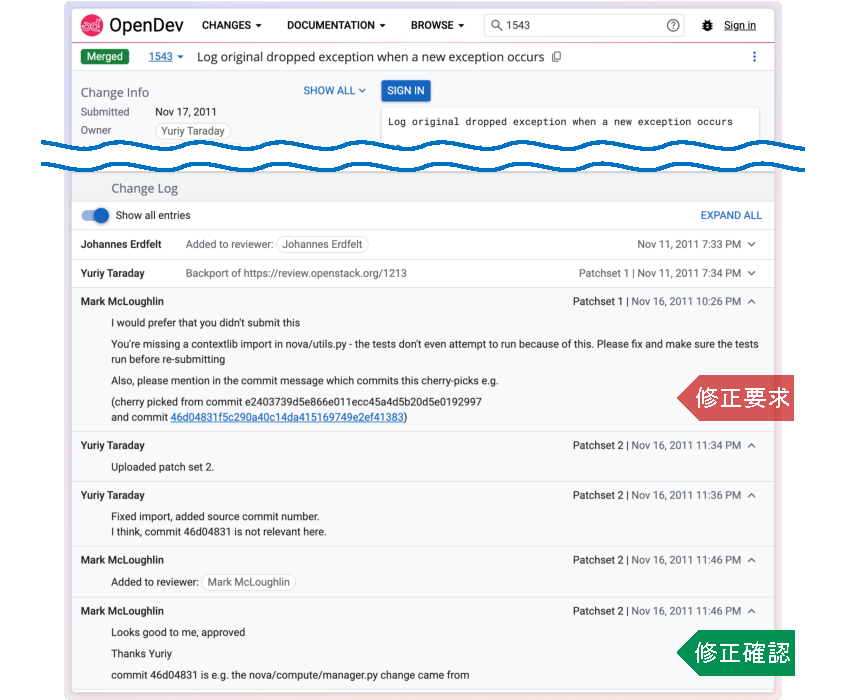
\includegraphics[width=1.0\linewidth]{@BSthesis2024_Kawasaki/BSthesis2024_Kawasaki_fig/code_review.pdf}}
\caption{Gerritのコードレビュー画面}
\label{fig:code_review}
\end{figure*}
%-------------------

また,コードレビューを通して検証者に導入の判断が行われた場合については,次回のリリースに含められるため,コードレビューはソフトウェア開発のリリースに重要な影響を与える.ソフトウェア開発プロジェクトでは,リリーススケジュールに合わせて図\ref{fig:milestone}のようにコードレビューを含めたマイルストーンが計画される.ただし,提出されたソースコードの修正の必要性について,他の検証者,または実装者同士で意見が対立し,コードレビューの時間が長期化することも多い\cite{review_time1}\cite{review_time2}.そのため,より正確なマイルストーンを計画するためにコードレビューに含まれる議論の内容を追跡することが望まれるが,OSS開発では日々膨大な量のソースコードが提出されるため,個々の議論の内容を追跡することは難しい.また,議論に含まれるレビューコメントが修正要求であるか否か,および修正要求が満たされているかを検証者に寄って確認されているか否かを判断するための指標が存在しないため,コードレビューのタスクの完了状況を自動で追跡することは容易ではない.

%-------------------
\begin{figure*}[t]
\centerline{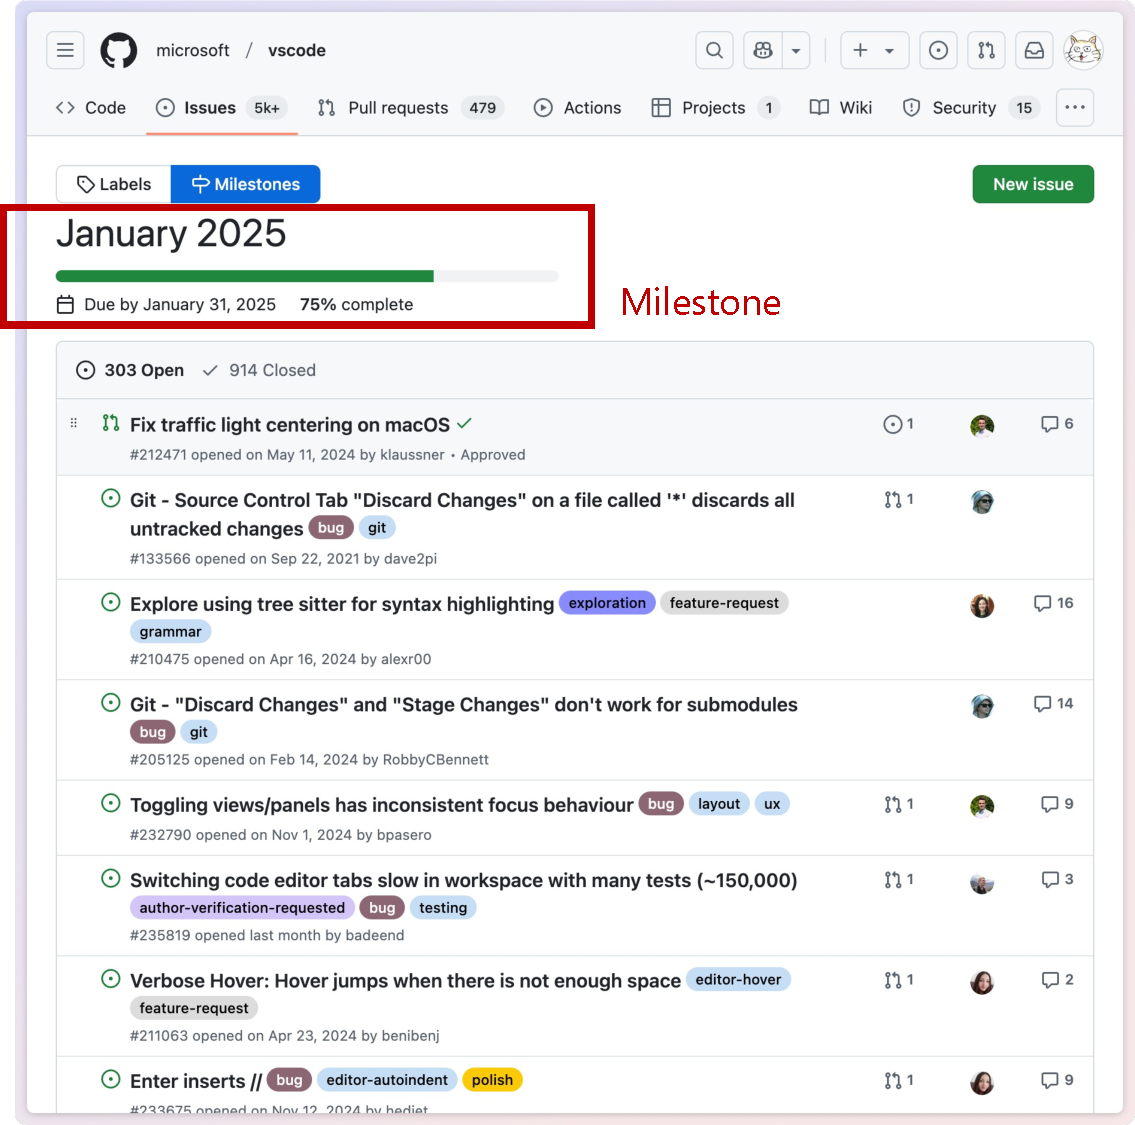
\includegraphics[width=0.9\linewidth]{@BSthesis2024_Kawasaki/BSthesis2024_Kawasaki_fig/milestone.pdf}}
\caption{GitHubのMilestoneの画面}
\label{fig:milestone}
\end{figure*}
%-------------------

\section{関連研究}
大規模OSSの開発では,実装者がコードレビュー依頼をGerritやReview Boardをはじめとしたコードレビュー管理システムの票に記録することで,実装者と検証者が円滑なコミュニケーションを行う~\cite{code_review}.これらのシステムに蓄積されたデータを用いて,コードレビューの作業内容や工数を見積もる研究が行われている.

大規模OSSの開発では,日々膨大なコードレビュー票がプロジェクトに提出されるため,開発者は優先して取り組むコードレビュー票に順位をつけて作業を効率化している.従来研究ではコードレビュー票の優先順位を決定するための研究が多数取り組まれており,ソフトウェア利用者に悪影響を与えるセキュリティ関連のソースコード変更のコードレビューは優先順位が高く設定されることが明らかにされている~\cite{integrator}\cite{review_prioritize_pineapple}.しかし,その他の急を要さない不具合修正やリファクタリングのために変更されたソースコードのコードレビューは優先順位が日々変動する\cite{review_priority_next_day}.

コードレビューの進捗を計画,追跡することは,リリースまでの緻密なマイルストーンを計画するために重要であり,各コードレビューに要する時間を見積もる研究が行われている.
Maddilaらは,レビューに参加している検証者の数やソースコードが提出された曜日など,レビューの完了時間に影響を与える要素を調査し,完了時間を予測するモデルを作成した\cite{estimate_time1}\cite{estimate_time2}.Chouchenらは,コードレビューに関する69個の要素から回帰分析を行い,レビューの完了時間を予測するモデルを作成した\cite{estimate_time3}.Jonathanらは検証者のレビューステータスを調査することでレビューにかかる時間を調査し,レビュー依頼を投稿したソースコード提案は依頼を投稿していないソースコード提案よりレビュー時間が短くなることを明らかにした\cite{estimate_time4}.Manoelらは,複数の回帰手法から最もレビュー時間の予測に適した手法を明らかにした\cite{estimate_time5}.Kononenkoらは,開発者へのインタビューにおいて,コード行数やコメントした検証者の数はコードレビューにかかる時間に影響を及ぼすことを明らかにした\cite{release_merge}.

従来研究ではコードレビューの優先順位,およびコードレビューにかかる工数の見積もりにコードレビューチケットを提出した時に計測できる特徴量に基づいていることが多い.本研究ではレビューコメント内で検証者によって投稿されている修正要求,および修正要求の完了度合いを抽出することで動的なタスクの完了状況の追跡を可能にする.

% \todo{SIGSEコピペ}
% 大規模OSSの開発では,実装者がコードレビュー依頼をGerritやReview Boardをはじめとしたコードレビュー管理システムの票に記録することで,実装者と検証者が円滑なコミュニケーションを行う~\cite{code_review}.これらのシステムに蓄積されたデータを用いて,コードレビューの作業内容や工数を見積もる研究が行われている.

% 大規模OSSの開発では,日々膨大なコードレビュー票がプロジェクトに提出されるため,開発者は優先して取り組むコードレビュー票に順位をつけざるを得ない.従来研究では,コードレビュー票の優先順位を決定するための研究が多数取り組まれており,ソフトウェア利用者に悪影響を与えるセキュリティ関連のソースコード変更のコードレビューは優先順位が高く設定されることが明らかにされている~\cite{integrator}\cite{review_prioritize_pineapple}.しかし,その他の急を要さない不具合修正やリファクタリングのために変更されたソースコードのコードレビューは優先順位が日々変動する.Kononenkoらは,開発者へのインタビューにおいて,直近のリリースに導入する変更提案の優先順位はリリースまでの期間によって異なることを明らかにしている\cite{release_merge}.

% コードレビューの進捗を計画,追跡することは,リリースまでの緻密なマイルストーンを計画するために重要であり,各コードレビューに要する時間を見積もる研究が行われている~\cite{estimate_time1}\cite{estimate_time2}\cite{estimate_time3}\cite{estimate_time4}\cite{estimate_time5}.
% Maddilaらは,コードレビュー対象のソースコード行数,変更内容の種類,コードレビューチケット作成日,ソースコード作成者の特徴など28の特徴量に基づきコードレビュー時間を見積もる手法を提案している\cite{estimate_time2}.

\section{動機}
ソフトウェア開発ではリリーススケジュールに合わせてマイルストーンを計画する.OSS開発では実装者から膨大な量のソースコードが提出されるため,従来研究ではコードレビューチケットが提出された時に優先順位や工数の見積もりを行う手法を提案している~\cite{estimate_time1}\cite{estimate_time2}\cite{estimate_time3}\cite{estimate_time4}\cite{estimate_time5}.しかし,コードレビューでは他の検証者や開発者同士で意見が対立することもあり,マイルストーンで予定していたコードレビューの時間を超過することも多い\cite{review_time1}\cite{review_time2}.本研究ではレビューコメントからタスクの完了状況を追跡するために,レビューコメントに含まれる修正要求の完了状況を自動で抽出することは可能であるかを調査する.

% \todo{SIGSEコピペ}
% コードレビューの優先順位,およびコードレビューにかかる工数の見積もりに関する従来研究では,コードレビューチケットを提出時に計測できる特徴量に基づいていることが多い.検証者による修正要求に基づき優先順位やコードレビューに要する時間を見積もることで,さらに正確なマイルストーンを計画することができると考える.そこで,本研究では修正要求コメント文を自動抽出する手法を開発し,コードレビューの進捗状況の追跡を試みる.

\section{リサーチクエスチョン}
本論文では,3つのRQを設定し,検証することで本研究の追跡手法がコードレビューのタスクの完了状況の追跡に有効であるかを評価する.

\vskip\baselineskip
\noindent\textbf{RQ1:\RQOne}

レビューコメントには提出されたソースコードに対する修正要求のコメント以外にも,他の開発者への質問や,修正要求が解決したことの確認など多種多様なコメントが投稿されている.そのため,レビューコメントから修正要求を高い精度で自動抽出することが可能であるかを調査する.

\vskip\baselineskip
\noindent\textbf{RQ2:\RQTwo}

RQ1と同様にレビューコメントには多種多様なコメントが投稿されているため,RQ2ではレビューコメントから修正確認を高い精度で自動抽出可能であるかを調査する.

\vskip\baselineskip
\noindent\textbf{RQ3:\RQThree}

コードレビューにおいて,開発者同士で意見が対立する場合は長期化することもあるため,従来手法のコードレビュー票を用いた手法では正確なタスクの完了状況を追跡することは難しい.本研究では,レビューコメントに含まれる修正要求を用いたタスクの完了状況追跡手法によって,従来のレビュー票に基づくタスクの完了状況追跡手法と評価結果が異なるかを調査する.

%%%%%%%%%%%%%%%%%%%%%%%%%%%%%%%%%%%%%%%%%%
%3章ケーススタディ
\chapter{ケーススタディ}\label{chap:case_study}
%%%%%%%%%%%%%%%%%%%%%%%%%%%%%%%%%%%%%%%%%%

\section{概要}
コードレビューでは複数の開発者からソースコードへの修正要求や,提出されたパッチへの問い,修正要求が解決したことの確認など多岐にわたるコメントが投稿されている.コードレビューにおけるタスクの完了状況の把握を行うためには,ソースコードに対する修正要求がどの程度完了しているかを抽出する必要がある.したがって,本研究ではレビューコメントの投稿数が多い,OpenStackのプロジェクトを対象にレビューコメントから修正要求と修正確認のコメントを抽出することでタスクの完了状況の追跡を行う.

本研究で用いる手法を図\ref{fig:research_method}に示す.まず,RQ1では検証者がコードレビューによって修正要求を依頼するコメント(修正要求コメント)をレビューコメントから抽出することが可能であるかを目視,及び自然言語処理モデルのBERTを用いて検証する.次に,RQ2ではソースコードが修正されたことを検証者によって確認されたことを伝えるコメント(修正確認コメント)をレビューコメントから抽出することが可能であるかを目視,及びパターンマッチを用いて検証する.最後に,RQ3ではRQ1のBERTで抽出した修正要求とRQ2のパターンマッチで抽出した修正確認を対応したコメント同士で紐づけることが可能であるかを検証する.これら3つのRQについて検証を行うことで,投稿された修正要求の完了度合いを把握し,コードレビューにおけるタスクの完了状況の追跡を可能とする.

% \todo{SIGSEコピペ(RQ1:修正要求/確認の目視)}
% コードレビュー票には多数のコメントが記録されている.実装者が投稿するコメントには,作成したソースコードの補足,検証者からの質問に対する回答などがある.検証者が投稿するコメントには,実装者への修正要求,提出されたパッチへの問い,修正要求が解決したことの確認などがある.RQ1では,コードレビュー票に記録されたコメントの中から,検証者がコードレビューによって更なる修正を依頼するコメント(修正要求コメント)か否か,ソースコードが修正されたことを検証者が確認したことを伝えるコメント(確認コメント)か否か,をそれぞれ分類できるか否かを目視調査する.

% \todo{SIGSEコピペ(RQ2:修正要求/確認の自動抽出)}
% RQ2では,RQ1で目視で抽出した修正要求コメント874件と修正確認コメント1,874件のデータセットを用いて,学習済みモデルBERTをファインチューニングし,レビューコメントに修正要求,および修正確認を含むか否かを機械的に特定するモデルを構築し,評価する.

% \todo{SIGSEコピペ(RQ3:レビュー票と修正要求の比較)}
% RQ2ではデータセットに対して修正要求と修正確認を抽出し,それぞれを対応したコメント同士で紐付けを行なった.RQ3では従来研究と同様にコードレビュー票の件数に基づき完了していないコードレビューの進捗状況を分析した結果と,修正要求の件数に基づいてコードレビューの進捗状況を分析した結果を比較する.

%-------------------
\begin{figure*}[t]
\centerline{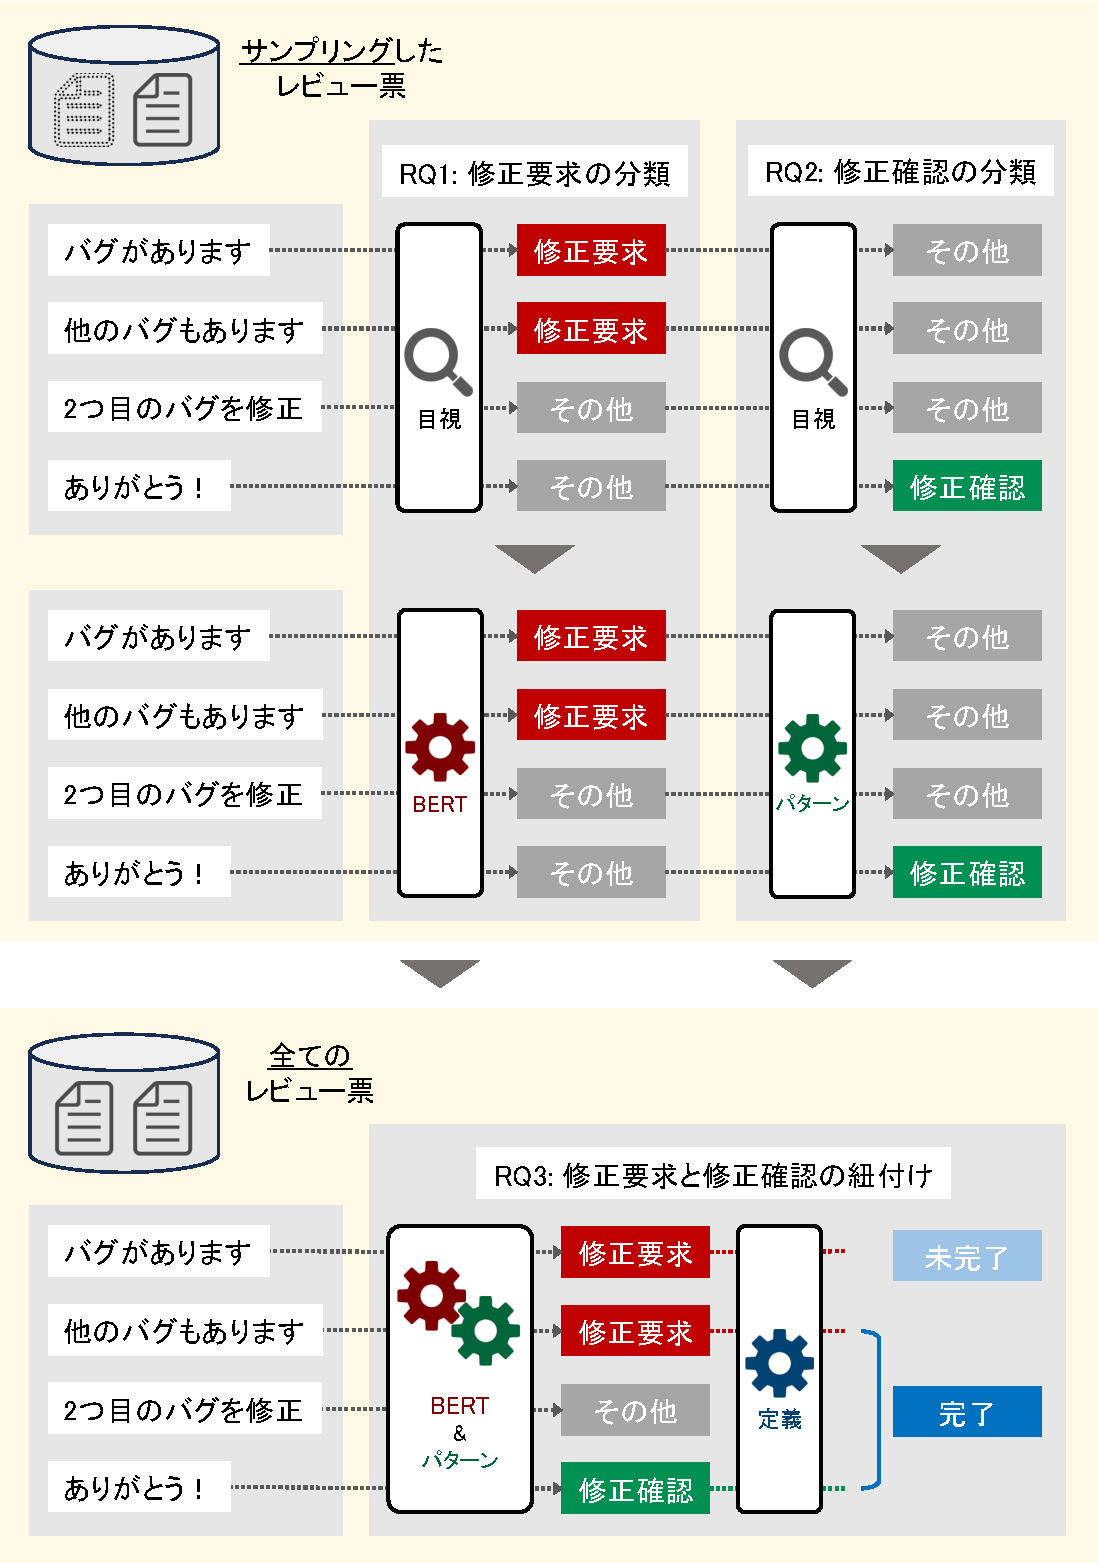
\includegraphics[width=1.0\linewidth]{@BSthesis2024_Kawasaki/BSthesis2024_Kawasaki_fig/research_method.pdf}}
\caption{コードレビューの進捗状況追跡手法}
\label{fig:research_method}
\end{figure*}
%-------------------

\section{データセット}
OpenStackプロジェクトでは,レビュー管理システムとしてGerritを使用しており,各コードレビュー票において開発者からのコメント投稿数が多いため,多くの従来研究がコードレビュー過程を分析する調査対象としている.そこで本研究では,OpenStackのコアコンポーネントであるNova,Neutron,Cinder,Keystone,Swift,Glanceの6つのプロジェクト,およびOpenStackにおける大規模プロジェクトであるHorizonの合計7つのプロジェクトのうち,プロジェクトの立ち上げから2023年5月までにリポジトリに導入されたコードレビュー票に記録されるコメントを分析対象とする.表\ref{table:sum_of_projects}は,各プロジェクトのコードレビュー票数,コメント数を示す.プロジェクト毎のコードレビュー票の平均コメント数は22件から87件であり,それぞれのコードレビュー票には多数のレビューコメントが投稿されていることが確認できる.

% \todo{SIGSEコピペ(RQ1:修正要求/確認の目視)}
% RQ1では,OpenStackのコアコンポーネントであるNova,Neutron,Cinder,Keystone,Swift,Glanceの6つのプロジェクト,およびOpenStackにおける大規模プロジェクトであるHorizonの合計7つのプロジェクトを分析対象とする.OpenStackプロジェクトでは,レビュー管理システムとしてGerritを使用しており,各コードレビュー票に開発者からのコメント投稿数が多いため,多くの従来研究がコードレビュー過程を分析する調査対象としている.本研究では,分析対象とするプロジェクトの立ち上げ時から2022年9月までにリポジトリに導入されたコードレビュー票に記録されるコメントを収集する.表\ref{table:NumberOfProjects}は,各プロジェクトのコードレビュー票数,コメント数を示す.プロジェクト毎のコードレビュー票の平均コメント数は22件から87件である.

%-----------------------
\begin{table}[t]
\centering
  \caption{各プロジェクトにおいて導入されたコードレビュー票数とコメント数}
  \vspace{+1mm}
  \label{table:sum_of_projects}
  \scalebox{1.0}{   
  \begin{tabular}{l|r|r}  \hline \hline
    \multicolumn{1}{c|}{プロジェクト} & \multicolumn{1}{c|}{コードレビュー票数} & \multicolumn{1}{c}{コメント数}\\ \hline
    Nova & 29,338 & 1,571,114\\ 
    Neutron & 18,665 & 1,106,829\\ 
    Cinder & 12,917 & 1,127,176\\ 
    Horizon & 9,645 & 209,681\\ 
    Keystone & 8,270 & 190,464\\ 
    Swift & 6,172 & 112,709\\ 
    Glance & 4,545 & 102,360\\ \hline
    合計 & 89,552 & 4,420,333\\ \hline
  \end{tabular}
  }
\end{table}
%-----------------------

%%%%%%%%%%%%%%%%%%%%%%%%%%%%%%%%%%%%%%%%%%
%4章 RQ1
\chapter{RQ1:\RQOne}\label{chap:RQ1}
%%%%%%%%%%%%%%%%%%%%%%%%%%%%%%%%%%%%%%%%%%

\section{概要}

\new{概要を追加}
RQ1では,本研究で用いるデータセットのうち無作為に選択した一部のコードレビュー票に記録されたコメントの中から,修正要求を抽出することが可能かを目視調査得する.また,目視調査にて修正要求には他のレビューコメントと異なる特徴が存在するということを確認した場合は,目視調査で作成した修正要求か否かを分類したデータセットを用いて,学習済みモデルのBERTをファインチューニングし,レビューコメントから修正要求を抽出するモデルを構築し,評価する.

\section{手法}
\subsection{目視での分類手法}

分析対象とする7プロジェクトを区別せずに89,552件のコードレビュー票から信頼区間95\%,許容誤差5\%となる383件を無作為に選択し,コードレビュー票に投稿されたコメント12,086件を目視調査する.具体的には,投稿されたコメントが修正要求のコメントか否かを分類する.ただし,ボットによるテスト実行結果は修正要求と判定しない.

% \todo{RQ1:修正要求/確認の目視}
% 分析対象とする7プロジェクトを区別せずに89,552件のコードレビュー票から信頼区間95\%,許容誤差5\%となる383件を無作為に選択し,コードレビュー票に投稿されたコメント12,086件を目視調査する.具体的には,修正要求のコメント,および修正確認のコメントを抽出する.ただし,ボットによるテスト実行結果は修正要求,修正確認と判定しない.

\subsection{BERTでの分類手法}

目視調査にてレビューコメントから修正要求を分類できる可能性を得た場合については,自然言語モデルBERT\footnote{BERT: \url{https://huggingface.co/docs/transformers/ja/model_doc/bert}}を,目視調査したデータセットを教師データとして用いてファインチューニングしたモデルでレビューコメントに修正要求を含むか否かを判定する.\todo{検証評価ラベルの詳細説明,ラベル削除時のBERTの説明を記述}目視調査した12,086件を5分割し,1つをテスト用のデータに用いて,残りの4つを訓練用のデータに用いる5分割交差検証を行う.訓練用のデータは,さらに7:3の割合で分割して学習用と検証用に用いる.モデル作成時のパラメータは学習時のパッチサイズが8,評価時のパッチサイズが16,エポック数が3,ウォームアップステップ数が500,重み減衰が0.01とした.評価指標には適合率,再現率,F1値を用い,交差検証で5回実行した結果の中央値でモデルの有用性を評価する.また,Gerritが提供する検証評価ラベルが分類に与える影響を確認するため,同様の設定のモデルでコメントからラベルを削除したコメントだけをテストデータに用いた評価も行う.

\todo{SIGSEコピペ(N-gramの話を加える)}
本研究の手法を図\ref{fig:research_method}に示す.コードレビューの進捗状況追跡のため,レビューコメントから修正要求及び修正確認を抽出する.まず,レビューコメントから修正要求を抽出するため,\ref{sec:RQ1}章で目視調査したデータセットを教師データとして用い,自然言語モデルBERT\footnote{BERT: \url{https://huggingface.co/docs/transformers/ja/model_doc/bert}}をファインチューニングしたモデルでレビューコメントに修正要求を含むか否かを判定する.目視調査した12,086件を5分割し,1つをテスト用のデータに用いて,残りの4つを訓練用のデータに用いる5分割交差検証を行う.訓練用のデータは,さらに7:3の割合で分割して学習用と検証用に用いる.モデル作成時のパラメータは学習時のパッチサイズが8,評価時のパッチサイズが16,エポック数が3,ウォームアップステップ数が500,重み減衰が0.01とした.評価指標には適合率,再現率,F1値を用い,交差検証で5回実行した結果の中央値でモデルの有用性を評価する.また,Gerriが提供する検証評価ラベルが分類に与える影響を確認するため,同様の設定のモデルをラベルを含むコメントからラベルを削除したコメントだけをテストデータに用いて評価を行う.

\section{結果}
\subsection{目視での分類結果}

\todo{SIGSEコピペ(内容はあまりいじらない予定)}
表~\ref{table:request_sum}および表\ref{table:achieve_sum}は,分析対象とする12,086件のコメントから修正要求コメントか否か,修正確認コメントか否か,を内容に基づき目視分類した結果を示す.

表~\ref{table:request_sum}の結果から,12,086件のレビューコメントのうち,874件(約7.2\%)が修正要求コメントであった.それぞれの修正要求コメントは5パターン(機能改善,リファクタリング,コード外の修正,バグ修正,誤字修正)に分類でき,検証者によって記述されることが多いパターンは機能改善,リファクタリング,コード外の修正であることを確認した.その他には,変更されたソースコードに欠陥が含まれるバグ修正や誤字修正の依頼が含まれていた.検証者によって記述された修正要求コメントには,表~\ref{table:request_sum}に示す他にも\textit{``Need a space before 5.''}や\textit{``This could use a bit more explanation in the commit message.''},\textit{``Please fix the pep8 errors''}のように\textit{``need''},\textit{``could''},\textit{``please''}などの自然言語で一般的に要求を表す単語が多く用いられていた.
Gerritでは,検証者がコードレビューのコメントに評価結果を表すラベルの付与を示す機能を有している.具体的には,変更内容に賛成していることを表すラベルとして\textit{``Looks good to me, approved(Code-Review+2)''}や\textit{``Looks good to me, but someone else must approve(Code-Review+1)''}などがある.また,変更内容に反対していることを表すラベルとして\textit{``I would prefer that you didn't submit this''}や\textit{``I would prefer that you didn't merge this''}などがある.ただし,たとえ変更内容に賛成していても修正要求を併記していることもある.本分析では変更内容に賛成していても修正要求が併記されているコメントを92件(約6%)を確認したため,検証評価ラベルのみで要求ありを分類することはできない.

これらの結果からレビューコメントにおける修正要求または修正確認には特徴があることを確認したため,修正要求や修正確認は機械的な手法でレビューコメントから抽出できることが示唆される.

%-----------------------
\begin{table*}[t]
\centering
  \caption{修正要求に含まれていた内容}
  \label{table:request_sum}
  \scalebox{0.8}{   
  \begin{tabular}{l|l|r}  \hline \hline
    \multicolumn{1}{c|}{修正要求内容} & \multicolumn{1}{c|}{コメント例} & \multicolumn{1}{c}{件数(重複可)}\\ \hline
    機能改善 & better to use mock instead of stub & 345\\ \hline
    リファクタリング/コード整形 & Could you use rstrip instead? & 278\\ \hline
    コード外の修正(コミットメッセージ等) & commit message line should have less than 72 characters & 233\\ \hline
    バグ修正 & need to address failures in unit tests & 92\\ \hline
    誤字修正 & fileds -\textgreater fields & 47\\ \hline
  \end{tabular}
  }
\end{table*}
%-----------------------

\subsection{BERTでの分類結果}

\todo{SIGSEコピペ(N-gramの結果を載せて,BERTの予測精度について考察を追加予定)}
表\ref{table:label_score}は,本研究でBERTをファインチューニングした予測モデルによって修正要求コメントを予測した結果を示す.5分割交差検証の結果,適合率が0.84,再現率0.78,F値0.81となった.この結果から修正要求コメントを高い精度で予測できることを明らかにした.現時点で,予測モデルの結果の比較対象となる手法を検討できていないため十分な有用性の評価を示すことができていないが,今後の研究では,自然言語として要求文を特定する既存手法との比較を検討する.

また,表\ref{table:label_score}には,Gerritが提供する検証評価ラベルを含むコメントからラベルを削除したコメントだけをテストデータに用いた評価結果も示す.Code-Review-1は修正要求を含むコメントが多量に存在するため,全ての評価指標で高いことがわかる.しかし,Code-Review+1やCode-Review+2では一般的に修正内容に賛同しているが,要求を併記していることもあるために再現率が低下したと示唆される.

%-----------------------
\begin{table}[t]
\centering
  \caption{修正要求コメントの予測精度}
  \label{table:label_score}
  \scalebox{1.00}{   
  \begin{tabular}{l|r|r|r}  \hline \hline
    \multicolumn{1}{c|}{スコア(件数)} & \multicolumn{1}{c|}{適合率} & \multicolumn{1}{c|}{再現率} & \multicolumn{1}{c}{F値}\\ \hline
    全レビューコメント(12,086件) & 0.84 & 0.78 & 0.81\\ \hline    
    Code-Review-2(14件) & 0.20 & 1.00 & 0.33\\ 
    Code-Review-1(465件) & 0.97 & 0.97 & 0.96\\ 
    Code-Review+1(918件) & 0.78 & 0.70 & 0.69\\ 
    Code-Review+2(916件) & 0.60 & 0.64 & 0.63\\ \hline
  \end{tabular}
  }
\end{table}
%-----------------------

次に,表\ref{table:request_accuracy}は,RQ1にて分類した修正要求内容別の再現率を示す.修正要求内容が200件以上存在する機能改善,リファクタリング/コード整形は,再現率が8割以上であることを確認した.
%それ以外の修正要求も7割以上ではあったが,コード外の修正依頼には表現にばらつきがあるため,再現率が落ちてしまったと示唆する.
また,コード外の修正やバグ修正,誤字修正の修正要求の再現率はすべて7割以上であるものの,機能改善やリファクタリング/コード整形と比べると再現率が低下した.この理由として,コード外の修正はコミットメッセージの修正や変更に対するパッチの分割要求など,修正要求の対象が多岐にわたっていることが起因していると示唆する.
%誤字修正は,RQ1の目視分析を通して他の修正要求より定型的な表現を用いられていることが多かったが,再現率が8割未満であり,データセットの中に誤字修正に関する要求が少ないことが起因していると示唆する.
また,バグ修正や誤字修正は,RQ1の目視分析を通して他の修正要求より定型的な表現を用いられていることが多かったが,データセットの中にバグ修正や誤字修正に関する要求が少ないことが再現率の低下に起因していると示唆する.

%-----------------------
\begin{table}[t]
\centering
  \caption{修正要求内容毎の再現率}
  \label{table:request_accuracy}
  \scalebox{1.1}{
  \begin{tabular}{l|r}  \hline \hline
    \multicolumn{1}{c|}{修正要求内容} & \multicolumn{1}{c}{再現率(\%)}\\ \hline
    機能改善 & 80.7\\ 
    リファクタリング/コード整形 & 85.3\\ 
    コード外の修正(コミットメッセージ等) & 75.5\\ 
    バグ修正 & 73.9\\ 
    誤字修正 & 78.7\\ \hline
  \end{tabular}
  }
\end{table}
%-----------------------

%%%%%%%%%%%%%%%%%%%%%%%%%%%%%%%%%%%%%%%%%%
%5章 RQ2
\chapter{RQ2:\RQTwo}\label{chap:RQ2}
%%%%%%%%%%%%%%%%%%%%%%%%%%%%%%%%%%%%%%%%%%

\section{概要}
\new{概要を追加}
コードレビューにおいて,修正要求が行われた箇所の修正が完了していた際,検証者は修正確認のコメントを投稿する.本章では,修正要求や質問など多種多様なコメントが投稿されているレビューコメントから修正確認を自動で抽出することは可能かを調査する.具体的にはレビューコメントを目視で修正確認か否かに分類し,得られた知見をもとに修正確認を抽出するためのパターンマッチを行う.

\section{手法}
\subsection{目視での分類手法}
RQ1と同様に本研究で用いるデータセットのうち信頼区間95\%,許容誤差5\%の383件のコードレビュー票に含まれる12,086件のレビューコメントにおいて目視で修正確認のコメントか否かを筆者が分類する.なお,コードレビューにおいては,ソースコードのビルド結果の確認など,自動化ボットによるコメントが含まれることがある.実装者がこれらボットのコメントに全て対処する前に検証者がソースコードを導入することもあるため,本研究ではボットによるコメントは修正確認の対象から除外する.

% \todo{RQ1:修正要求/確認の目視}
% 分析対象とする7プロジェクトを区別せずに89,552件のコードレビュー票から信頼区間95\%,許容誤差5\%となる383件を無作為に選択し,コードレビュー票に投稿されたコメント12,086件を目視調査する.具体的には,修正要求のコメント,および修正確認のコメントを抽出する.ただし,ボットによるテスト実行結果は修正要求,修正確認と判定しない.

\subsection{パターンマッチでの分類手法}
2つの定義のいずれかに該当する語彙を含むレビューコメントを修正確認として抽出するパターンマッチを行う.

\begin{itemize}
\item 修正確認と分類されたコメントの中に含まれる語彙を抽出し,その語彙が含まれるコメントにおいて,修正確認と分類された割合が90\%を超えた語彙
\item Gerritで手供されているコードレビュー結果の承認を示す語彙
\end{itemize}

% \todo{SIGSEコピペ(修正要求/確認の自動抽出)}
% 図\ref{fig:research_method}に示すようにレビューコメントから修正確認を抽出する.修正確認は修正要求と異なり言語的表現が少なく,Gerritで提供されているコードレビューの結果を示すラベルや``LGTM''のように定型的な表現がなされていることが多い.そこで表\ref{table:achieve_sum}の「その他」に分類した語彙を含むコメントを抽出したところ,\textit{``LGTM''},\textit{``Looks good''},\textit{``Looks ok''}を含むコメントのみレビューコメントを修正確認と分類した割合が90\%を超えていることを確認した.そこで本研究での修正確認として用いるコメント群は表\ref{table:achieve_sum}で示す強い承認,弱い承認つまり,Gerritで提供されているコードレビュー結果のスコア及び\textit{``LGTM''},\textit{``Looks good''},\textit{``Looks ok''}を含むコメントとする.

\section{結果}
\subsection{目視での分類結果}
表\ref{table:achieve_sum} は,分析対象とする12,086件のコメントから修正確認コメントか否か,を内容に基づき目視分類した結果を示す.12,086件のレビューコメントのうち,1,874件(約15.5\%)が修正確認コメントであった.1,874件の修正確認コメントのうち,1,559件(約83.2\%)はOpenStackで提供されている変更提案に対する承認を表すラベルがレビューコメントに付与されていることを確認した.また,検証評価ラベル以外の修正確認コメントとして,\textit{``Good Change``}や\textit{``Thank you``}などの感謝を示すコメントを投稿する検証者も複数確認した.

この結果からレビューコメントにおける修正確認には特徴があることを確認したため,修正確認は機械的な手法でレビューコメントから抽出できることが示唆される.

% \todo{SIGSEコピペ(RQ1:修正要求/確認の目視)}
% 表~\ref{table:request_sum}および表\ref{table:achieve_sum}は,分析対象とする12,086件のコメントから修正要求コメントか否か,修正確認コメントか否か,を内容に基づき目視分類した結果を示す.

% 次に表\ref{table:achieve_sum}の結果から,12,086件のレビューコメントのうち,1,874件(約15.5\%)が修正確認コメントであった.1,874件の修正確認コメントのうち,83.2\%はOpenStackで提供されている変更提案に対する承認を表すラベルがレビューコメントに付与されていることを確認した.また,検証評価ラベル以外の修正確認コメントとして,\textit{``Good Change''}や\textit{``Thank you''}などの感謝を示すコメントを投稿する検証者も複数確認した.

% これらの結果からレビューコメントにおける修正要求または修正確認には特徴があることを確認したため,修正要求や修正確認は機械的な手法でレビューコメントから抽出できることが示唆される.

%-----------------------
\begin{table*}[t]
\centering
  \caption{修正確認に含まれていた内容}
  \label{table:achieve_sum}
  \scalebox{0.85}{   
  \begin{tabular}{l|l|r}  \hline \hline
    \multicolumn{1}{c|}{修正確認内容} & \multicolumn{1}{|c}{コメント} & \multicolumn{1}{|c}{件数(重複無)} \\ \hline
    強い承認 & Looks good to me, approved または Code-Review+2 & 666 \\ \hline
    弱い承認 & Looks good to me, but someone else must approve または Code-Review+1 & 893 \\ \hline
    その他 & Good Change や Thank you や Nice など & 315 \\
    % & I would prefer this is not submitted as is または \\ Code-Review-1 & 弱い非承認 \\ \hline
    % This shall not be submitted または \\ Code-Review-2& 強い非承認 \\ 
    \hline
  \end{tabular}
  }
\end{table*}
%-----------------------

\subsection{パターンマッチでの分類結果}
目視調査にて修正確認と分類されたコメントの中に含まれる語彙を抽出したところ,\textit{``LGTM``},\textit{``Looks good``},\textit{``Looks ok``}を含むコメントのみレビューコメントを修正確認と分類した割合が90\%を超えていることを確認した.そこで本研究での修正確認として用いるコメント群は表\ref{table:achieve_sum}で示す強い承認,弱い承認及び\textit{``LGTM``},\textit{``Looks good``},\textit{``Looks ok``}を含むコメントとする.

表\ref{table:achieve_score}は,本研究で修正確認コメントを特定するとして用いる基準による結果を示す.評価実験の結果,再現率が97\%であった.\textit{``LGTM``}以外にも\textit{``Thank you``}による修正確認もあるが,修正確認以外にも使われる用語のため,再現率が100\%に至っていない.

% \todo{SIGSEコピペ(RQ2:修正要求/確認の自動抽出)}
% 表\ref{table:confirm_score}は,本研究で修正確認コメントを特定するとして用いる基準による結果を示す.評価実験の結果,再現率が97.3\%であった.\textit{``LGTM''}以外にも\textit{``Thank you''}による修正確認もあるが,修正確認以外にも使われる用語のため,再現率が100\%に至っていない.

%-----------------------
\begin{table}[t]
\centering
  \caption{修正確認コメントの予測精度}
  \label{table:achieve_score}
  \scalebox{1.00}{   
  \begin{tabular}{l|r|r|r}  \hline \hline
    \multicolumn{1}{c|}{スコア(件数)} & \multicolumn{1}{c|}{適合率} & \multicolumn{1}{c|}{再現率} & \multicolumn{1}{c}{F値}\\ \hline
    全レビューコメント(12,086件) & 0.94 & 0.97 & 0.96\\ \hline    
  \end{tabular}
  }
\end{table}
%-----------------------

%%%%%%%%%%%%%%%%%%%%%%%%%%%%%%%%%%%%%%%%%%
%6章 RQ3
\chapter{RQ3:\RQThree}\label{chap:RQ3}
%%%%%%%%%%%%%%%%%%%%%%%%%%%%%%%%%%%%%%%%%%

\section{概要}
\new{概要を追加}
RQ3では,RQ1とRQ2でBERTおよびパターンマッチを用いて修正要求と修正確認を高い精度で抽出可能ということを確認した場合に,本研究で用いるデータセット全てを用いて修正要求と修正確認を対応したコメント同士で紐づけることができるのかを検証する.また,従来手法の完了していないコードレビュー票の件数に基づいたコードレビューのタスクの完了状況を分析した結果と,修正要求の件数に基づいてコードレビューのタスクの完了状況を分析した結果を比較する.

\section{手法}
\subsection{修正要求と修正確認の紐付け手法}
\new{紐付け手法を追加}
検証者は,修正要求に基づいて修正されたソースコードを確認したとき,修正確認を投稿することがある.しかし,RQ1の目視調査において修正要求に対する修正確認が投稿されているか否かを確認したところ,必ずしも修正要求を投稿した検証者が修正確認を投稿しているとは限らないことがわかった.また,複数の検証者が異なる修正要求コメントを投稿し,ソースコードが修正された後に,いずれか1人の検証者が全ての要求に対する修正が完了していることを確認していることもある.

そこで本研究ではタスクの完了状況評価を行うために,図\ref{fig:research_method}に示す修正要求と修正確認の紐付けには修正要求と後のパッチで投稿された修正確認を2つの定義で行う.

\begin{itemize}
\item 修正確認コメントを投稿した検証者が,以前に投稿した要求は全て検証されたものとみなす
\item 修正確認コメントの投稿以前の要求は全て検証されたものとみなす
\end{itemize}

% \todo{SIGSEコピペ(内容はあまり変える予定なし)}
% 修正要求に基づき修正されたソースコードが確認されたとき,検証者は修正確認コメントを投稿することがある.しかし,RQ1で目視によって修正要求に対する修正確認が投稿されているか否かを確認したところ,必ずしも修正要求コメントを投稿した検証者が,修正確認コメントを投稿しているとは限らないことがわかった.また,複数人の異なる検証者が修正要求コメントを投稿し,ソースコードが修正された後に,いずれか一人の検証者が全ての要求に対する修正が完了していることを確認していることもある.

% そこで本研究では進捗状況評価を行うための第一歩として,図\ref{fig:research_method}に示す修正要求と修正確認の紐付けには修正要求と後のパッチで提出された修正確認を2つの定義で行う.
% \begin{itemize}
% \item 修正確認コメントを投稿した検証者が,以前に投稿した要求は全て検証されたものとみなす
% \item 修正確認コメントを投稿以前の要求は全て検証されたものとみなす
% \end{itemize}

\subsection{レビュー票と修正要求の比較手法}
\new{比較手法を追加}
RQ1で抽出した修正要求コメント239,286件に対して,1日毎に完了していない(GerritのStatusがMergeやAbandonedでない)コードレビュー票の件数とRQ2

\todo{SIGSEコピペ(内容はあまり変える予定なし)}
RQ2で抽出した修正要求コメント239,286件に対して,1日毎に完了していない(GerritのStatusがMergedやAbandonedでない)コードレビュー票の件数とRQ2で定義した修正確認コメント「修正確認コメントを投稿以前の要求は全て検証されたものとみなす」に基づき,修正確認されていない修正要求の件数の分布を分析する.ただし,修正確認と紐づかなかった修正要求はその修正要求を含む変更提案が導入された時点で修正要求は満たされたこととする.

\section{結果}
\subsection{修正要求と修正確認の紐付け結果}
\todo{SIGSEコピペ(内容はあまり変える予定なし)}
表\ref{table:link_ratio}は,89,552件の変更提案から239,286件の修正要求を抽出し,4.2.3項で定義した方法で修正要求と修正確認とを紐付けた結果を示す.修正要求提出者が後のパッチで修正確認を行うことは4割程度であり,多くの検証者が修正要求に対して改修後,修正確認コメントを投稿していないことが示唆される.ただし,検証者を問わなければ約8割で修正確認が行われていることが示唆される.

%-----------------------
\begin{table}[t]
\centering
  \caption{定義毎に修正要求(239,286件)と紐づいた割合}
  \label{table:link_ratio}
  \scalebox{1.2}{   
  \begin{tabular}{l|r|r}  \hline \hline
    \multicolumn{1}{c|}{紐付けの定義} & \multicolumn{1}{c|}{件数} & \multicolumn{1}{c}{割合(\%)}\\ \hline
    修正要求提出者が修正確認 & 110,042 & 45.8\\ 
    検証者を問わず修正確認 & 207,997 & 86.6\\ \hline
  \end{tabular}
  }
% \end{table}
% %-----------------------
% %-----------------------
% \begin{table}[t]
\centering
  \caption{プロジェクト毎の1日あたりの変更提案数と修正要求数の分布}
  \label{table:Mann-White}
  \scalebox{1.2}{   
  \begin{tabular}{l|r}  \hline \hline
    \multicolumn{1}{c|}{プロジェクト} & \multicolumn{1}{c}{p値}\\ \hline
    Neutron & 1.14e-40\\ 
    Nova & 5.60e-39\\ 
    Glance & 5.14e-07\\ 
    Cinder & 2.81e-18\\ 
    Swift & 2.78e-64\\ 
    Horizon & 5.87e-07\\ 
    Keystone & 1.15e-05\\ \hline
  \end{tabular}
  }
\end{table}
%-----------------------

\subsection{レビュー票と修正要求の比較結果}


\todo{SIGSEコピペ(p値が高いプロジェクトに変更.また,考察でプロジェクト毎の違いを議論する場合は付録にそれぞれのグラフを添付する可能性あり)}
図\ref{fig:task_dist}は,1日毎に存在したコードレビュー票の件数と修正要求の件数の分布を示す.NeutronやCinder,Keystoneは他のプロジェクトと比較しても特に中央値や外れ値の分布がコードレビュー票と修正要求で分布が異なっている.表\ref{table:Mann-White}はプロジェクト毎の1日あたりの変更提案数と修正要求数を有意水準は5\%としてMann-WhitneyのU検定の結果を示す.全てのプロジェクトの分布で統計的に有意な差があり,1つのコードレビューにおいて修正要求コメントが複数存在していることが多い.したがって,コードレビュー票の件数のみでリリーススケジュールを立案すると,期待よりも修正要求数が多いコードレビュー票において誤差が生じることが示唆される.

図~\ref{fig:task_trans}は,一例としてKeystoneプロジェクトを対象に,検証が完了していないコードレビュー票数の推移と,修正確認されていない修正要求数の推移を示す.図~\ref{fig:task_trans}から,2011年から2014年,2018年から2020年では,検証が完了していないコードレビュー票数と修正確認されていない修正要求数がほぼ同じであるため,コードレビュー票1件に修正要求が1件程度であることが示唆される.一方で,それ以外の2015年から2017年ではコードレビュー票1件に対して修正要求が2件以上であることが示唆される.この時期は,修正要求数が多い時期であったことがわかる.ただし,本研究では修正要求の修正にかかる時間的コストや修正の難しさを考慮できていない.今後は,修正要求の修正にかかるコストを考慮することで,リリーススケジュールへの影響を明らかにできると考える.


%-------------------
\begin{figure}[t]
\centerline{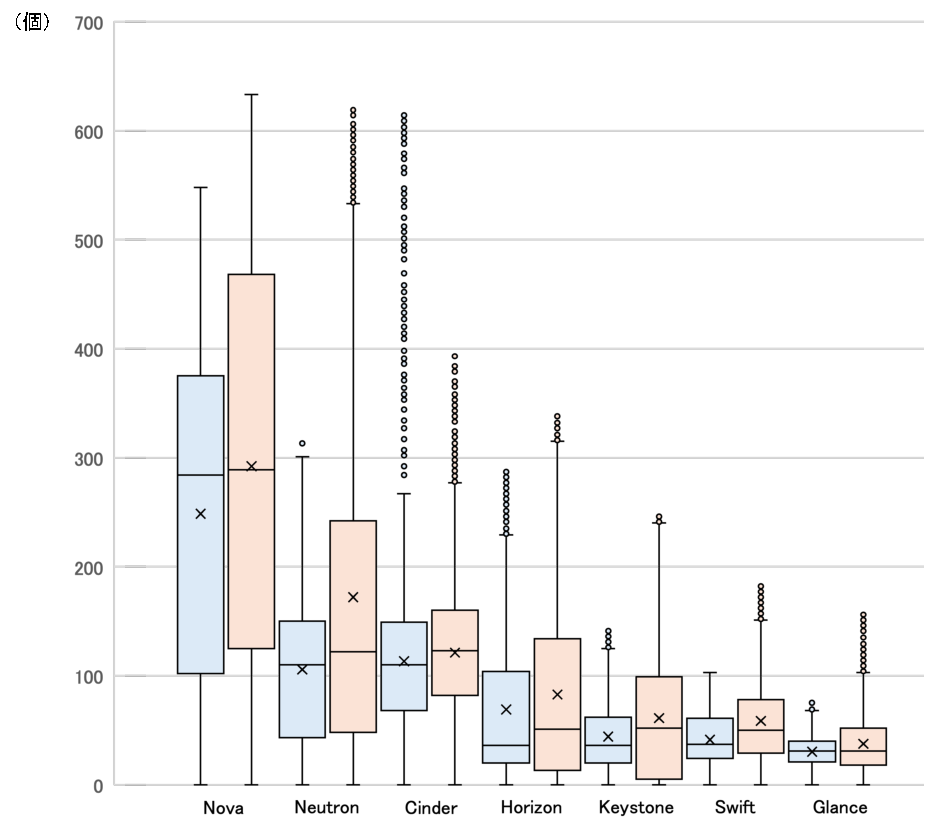
\includegraphics[width=1.0\linewidth]{@BSthesis2024_Kawasaki/BSthesis2024_Kawasaki_fig/task_dist.pdf}}
\caption{1日毎の存在するコードレビュー票の件数と修正要求の件数の分布(左:コードレビュー票, 右:修正要求)}
\label{fig:task_dist}

\vspace{2mm}

\centerline{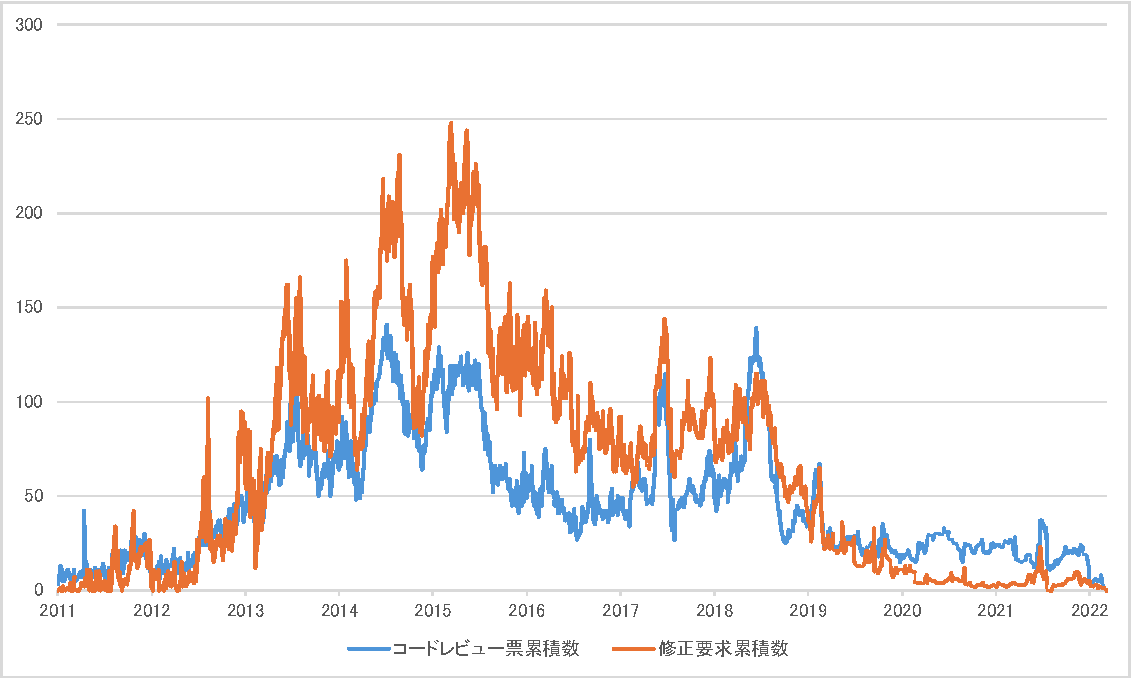
\includegraphics[width=1.0\linewidth]{@BSthesis2024_Kawasaki/BSthesis2024_Kawasaki_fig/task_trans.pdf}}
\caption{Keystoneのコードレビュー票と修正要求の開放数の推移}
\label{fig:task_trans}
\end{figure}
%-------------------

%%%%%%%%%%%%%%%%%%%%%%%%%%%%%%%%%%%%%%%%%%
%7章 考察
\chapter{考察}\label{chap:discussion}
%%%%%%%%%%%%%%%%%%%%%%%%%%%%%%%%%%%%%%%%%%

\section{レビュー票と修正要求の開放数に差異が生じた原因}
\todo{プロジェクト間,pythonプロジェクトの変遷,コードレビューの歴史etc..とかを考察できたらいいな}

\section{妥当性の脅威}
\subsection{内的妥当性}
\todo{SIGSEコピペ(内容はあまり変える予定なし)}
本研究ではレビューコメント修正要求か否か,修正確認か否かを著者が目視によって判断している.目視による分類結果は,他者の評価基準によって分類が異なる可能性がある.今後は複数人による目視分類を実施することで,分類の信頼度の向上させる.

また,修正確認の定義としてGerritで提供されているコードレビュー結果のスコア及び\textit{``LGTM''},\textit{``Looks good''},\textit{``Looks ok''}を含むコメント群を用いたが,実際には\textit{``Good Change''}や\textit{``Thank you''}のような他の表現を用いた修正確認が存在する.しかし,定義した修正確認コメント群は著者が分類した修正確認のうちF値が0.96と高い値であることから他の表現による修正確認による影響は小さいと示唆される.

また,紐付けの定義として二つの定義を提示したが,実際には定義に基づかない紐付き方も存在する.しかし,修正確認コメントが高い割合で抽出可能なことから紐付き方による影響は小さいと示唆する.

\subsection{外的妥当性}
\todo{SIGSEコピペ(内容はあまり変える予定なし)}
本研究では,OpenStackのコアコンポーネントの6つのプロジェクトと大規模プロジェクトであるHorizonを対象とした.対象として用いるプロジェクトや期間によっては予測精度や分析結果が異なることが示唆される.しかし,OpenStackプロジェクトでは,各コードレビュー票に開発者からのコメント投稿数が多いため,データセットとするプロジェクトや期間の変更による予測精度や分析結果への影響は小さいと示唆する.

%%%%%%%%%%%%%%%%%%%%%%%%%%%%%%%%%%%%%%%%%%
%8章 おわりに
\chapter{おわりに}\label{chap:conclusion}
%%%%%%%%%%%%%%%%%%%%%%%%%%%%%%%%%%%%%%%%%%

\todo{SIGSEコピペ(N-gramの結果や考察等が追加されるので内容は大きく変わる可能性あり.方向性は変えないけど)}
本研究では,コードレビュー票に記録される修正要求コメント,および修正確認コメントに基づく進捗状況を把握する手法を提案し,3つのRQを検証した.その結果,BERTを用いた手法で修正要求を高い精度で抽出可能であることを確認した.また,1件のコードレビューにおいて,複数の修正要求を含んでいることが多く,コードレビュー票の件数のみでリリーススケジュールを立案すると,期待よりも修正要求数が多いコードレビュー票において誤差が生じることが示唆される.

今後は,修正要求コメントの詳細な分析を行い,多様な修正要求コメントを抽出可能なモデル構築を目指す.

また,進捗状況を追跡するためには修正にかかる時間的コストや修正の難しさを考慮する必要があるため,修正要求を種類毎に分類する手法の確立も目指す.

\begin{acknowledgements}
本研究を進めるに当たって,多くの方々から御指導,御協力を賜りましたことを,ここに深く感謝を申し上げます.

まず,指導教員である和歌山大学システム工学部伊原紀准教授に,心より感謝申し上げます.研究室配属から現在に至るまで,研究の方向性,論文執筆の作法,学会発表など,数多くの御指導を賜りました.また,研究発表の機会を与えてきたいただき,多くの研究者との貴重な交流の場を設けていただきました.ここに深く感謝の意を表します.

次に,本研究を進めるにあたり,多大なご協力をいただきました和歌山大学システム工学研究科上中瑞稀氏に厚く御礼申し上げます.研究に関して,御協力,御助言をいただきました.

また,和歌山大学ソーシャルソフトウェア工学研究室の方々には,普段から多大な御協力,御助言をいただきました.特に,ソーシャルソフトウェア工学研究室の同期の皆様には,研究面だけでなく,学生生活全般にわたって御支援いただき,充実した研究生活を送ることができました.心より感謝申し上げます.

最後に,長きにわたる研究生活を常に支え,励まし続けてくれた家族に対し,深い感謝の意を表します.

% まず、この研究の成功を支える全知全能の指導教員であり、私に「隠された力」を見出してくださった伊原教授に感謝申し上げます。もしも私が異世界に転生するようなことがあれば、必ずや教授の英知を魔法に応用し、無双の力を発揮することでしょう。教授のご助言は、私の研究という「ステータス」を何段階も引き上げてくれるものでした。

% また、この研究を進めるにあたり、魔王軍(読んで:研究の課題)との激闘を共に乗り越えた十協力者の皆様十に、深い感謝を捧げます。彼らとの議論や意見交換は、私の「スキル」を磨き上げ、最強の「パーティー」を形成するきっかけとなりました。

% さらに、本研究を支えてくださった秘密結社には、まさに異世界での「神からのギフト」のようなご支援をいただきました。おかげで、私の「知識のレベルアップ」が実現しました。この場を借りて厚く御礼申し上げます。

% 最後に、私が何度も「悪役令嬢」さながら研究の迷宮に迷い込んだ際も、優雅に手を差し伸べ、支えてくださった家族や友人に心より感謝いたします。皆様の愛情と応援は、まさに「ヒロインのピンチを救う騎士」のごときものでした。

% すべての皆様に、この研究という「勇者の冒険譚」の一頁を完成させる力を与えていただいたことを、改めて感謝申し上げます。そして、これからも新たなステージで「おれつえー」と自負できる成果を追い求めていく所存です。
\end{acknowledgements}

%================
%\section*{参考文献}
%================
\bibliographystyle{junsrt}
\bibliography{@BSthesis2024_Kawasaki/BSthesis2024_Kawasaki}

\end{document}
